\section{背景}
\subsection{无人机}
%%无人机行业发展
\frame {
	\frametitle{无人机行业发展}
	近几年国内无人机市场规模飞速发展,
	兴起了一批如大疆科技、零度智控等科技企业。
	\begin{figure}
		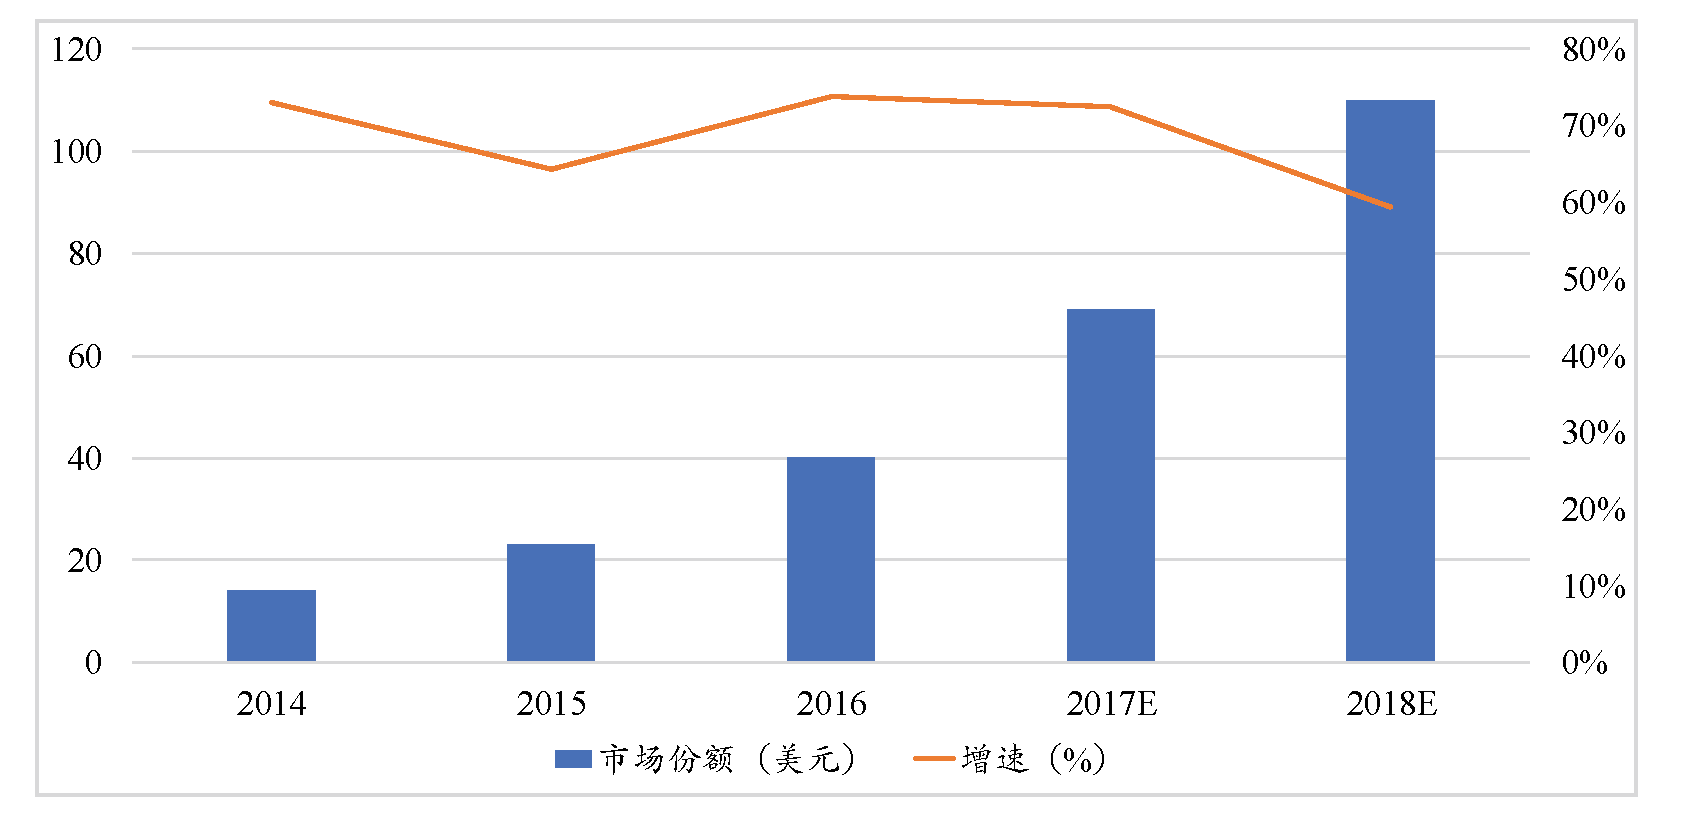
\includegraphics[height=4cm]{figures/uavshichang.eps}
		\caption{中国无人机市场规模}
		\label{fig:uavshichang}
	\end{figure}
}
%%无人机航拍
\begin{frame}[t]
	\frametitle{无人机航拍}
	\begin{columns}[t,onlytextwidth]
		%%左边列
		\begin{column}{0.6\textwidth}
		无人机一项重要应用是航拍。
		航拍所采用的数据传输方案很大程度上影响用户的体验。
		\vspace{1em}
		\begin{block}{视频传输方案}
			\footnotesize
			\begin{enumerate}[(1)]
				\item 专有数据链,如DJI的Lightbridge
				\item 基于TCP/IP的网络视频传输
			\end{enumerate}
		\end{block}
		%%右边列
		\end{column}
		\hspace{0.5em}
		\begin{column}{0.4\textwidth}
			\vspace{-3em}
			\begin{figure}
				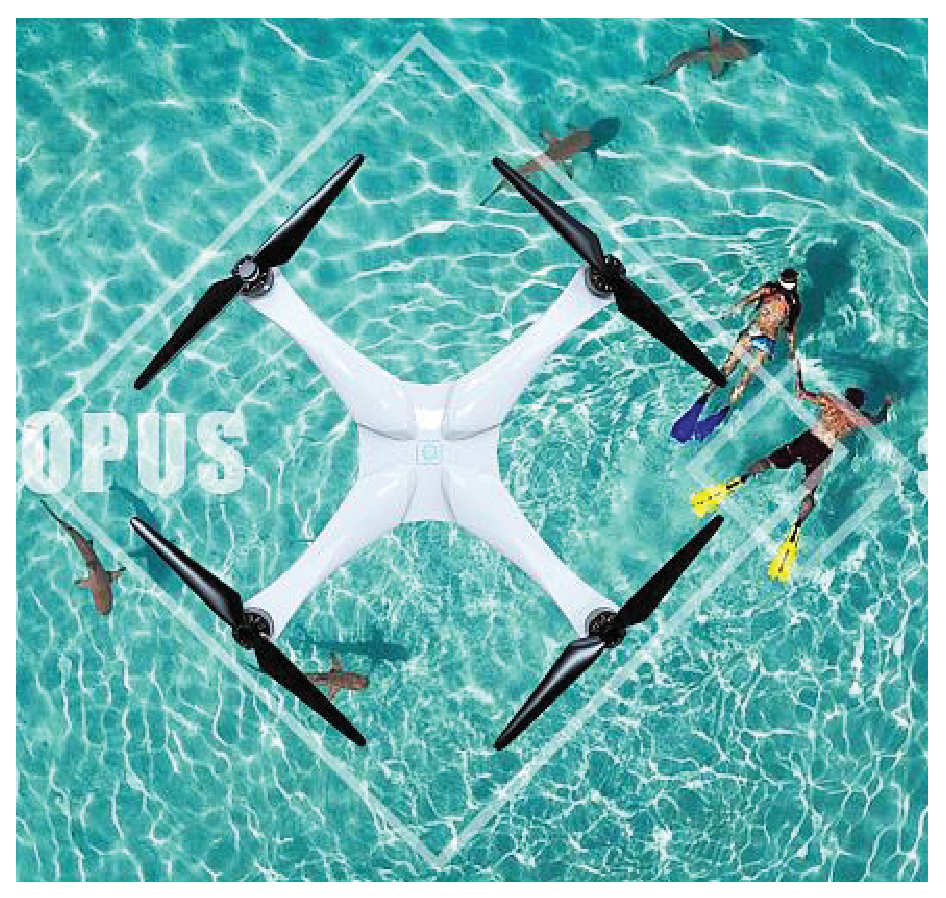
\includegraphics[height=4.2cm]{figures/uavhangpai.eps}
			\end{figure}
		\end{column}	
	\end{columns}
	%%新的一行
	\vspace{1.5em}
	两种传输方案都有各自的优缺点。
\end{frame}
%%两种视频传输方案优缺点
\frame {
	\frametitle{两种视频传输方案优缺点}
	
	\begin{columns}[t]
		%%左边列
		
		\begin{column}{0.4\textwidth}
			\begin{block}{专有数据链}
				\footnotesize
				\begin{block}{优点}
				传输时延小、单向广播
				\end{block}
				\begin{block}{缺点}
				需要专门设备,
				价格较高,
				且与目前因特网体系架构不兼容
				\end{block}
			\end{block}
		\end{column}
		%%右边列
		\begin{column}{0.55\textwidth}
			\begin{block}{基于TCP/IP的方案}
				\footnotesize
				\begin{block}{优点}
				与现有网络体系架构兼容,
				符合未来万物互联的趋势,
				设备价格低廉。
				\end{block}
				\begin{block}{缺点}
				传输时延大,
				容易受到无线链路中各种干扰,
				\color{red}{受限于TCP协议的缺点}。
				\end{block}
			\end{block}
		\end{column}
	\end{columns}
	\note{
		本文也是着眼于TCP协议的缺点,
		对TCP进行改进,
		以提高基于TCP协议的无人机视频传输的性能
	}
}

\subsection{TCP协议}
%%TCP简单概述
\frame {
	\frametitle{TCP简单概述}
	\begin{block}{TCP协议}
		\footnotesize
		TCP是一种可靠的面向连接的协议。
		为了保证其可靠性,
		设计了ACK确认机制,
		流控机制,
		拥塞控制算法。\\
		\begin{description}
			\item[ACK机制] 对于发送端发出的报文,
			如果接收端确实收到,那么会回复一个ACK报文进行累积确认。
			\item[流控机制] 为了让发送端的发送速度和接收端的接收速度匹配,
			接收端通过ACK报文中的\emph{接收窗口}字段告知发送端自己的处理能力,
			以让发送端调节好发送速度。
			\item[拥塞控制算法] 如慢启动、拥塞避免、快速重传和快速回复等,
			目的是当网络出现拥塞的时候,减慢发送速度,以避免网络进一步拥塞;
			当网络通畅的时候,增大发送速率,以最大化利用网络带宽。
		\end{description}

	\end{block}
}
%%使用TCP进行无人机视频传输存在的问题
%\begin{frame}[t]
\frame{
	\frametitle{使用TCP进行无人机视频传输存在的问题}
	TCP协议最初是针对有线网络设计的,
	考虑到有线网络中极低的误码率,
	其拥塞控制模型以丢包为基础。
	但无人机视频传输有其自身特点
	\begin{block}{无人机视频传输环境特点}
		\footnotesize
		大尺度衰落信道环境、
		多径干扰导致的高误码率;
		障碍物遮挡、基站切换导致的连接短暂中断;
		视频传输对传输时延很敏感。
	\end{block}
	标准TCP在面对这些特点时,表现出了天生的劣势。
	\begin{block}{劣势}
		\footnotesize
		\begin{enumerate}[(1)]
			\item 无法区分拥塞丢包和非拥塞丢包,
			频繁启动拥塞控制算法,
			降低发送速率。
			\item TCP的重传确保了可靠,但一定程度上增大了传输时延,而视频传输对时延很敏感。
		\end{enumerate}
	\end{block}
	\note{
		考虑到需要进行可靠传输,
		TCP的ACK机制是必要的,
		我们只能在减少重传次数上做文章。
		针对TCP无法区分拥塞丢包和非拥塞丢包问题上,
		以前的一些学者进行了相关改进。
		对于拥塞,如果将来将无人机接入到因特网中去,
		将是一个需要考虑的问题。
	}
}
%\end{frame}
%%如何克服这些缺点?
\begin{frame}[t,allowframebreaks]{如何克服这些缺点?}
	在处理拥塞丢包和非拥塞丢包问题上,
	有两种思想:掩盖非拥塞丢包和区分两种丢包。
	\vspace{1em}
	\begin{block}{掩盖非拥塞丢包}
		\begin{description}
			\footnotesize
			\item[ARQ] 应用于无线网络的链路层,
			但会和TCP的原有机制冲突,
			导致乱序。
			\item[FEC] 将前向纠错码和TCP结合,
			如使用异或运算对前\emph{n}个报文编码。
			\item[Indirect-TCP] 在有损信道入口处终止原始TCP连接,
			由TCP-agent接管报文。
			\item[TCP-snoop] 保持端到端语义,保存经过的数据的拷贝,处理重复ACK。
		\end{description}
	\end{block}
	\begin{block}{区分丢包}
		\footnotesize
		\begin{description}
			\item[ELN] 接收端的MAC层可以检测出错,
			将这一信息告知上层TCP,上层TCP会发送给对方一个报文告知出错。
			\item[TCP-vegas] 让拥塞检测和丢包解耦。但其同样无法处理丢包引起的重传导致的时延过大问题。
			\item[ECN] 显示拥塞控制标志位。利用IP首部的TOS字段。
		\end{description}
	\end{block}
	Sundararajan等人提出TCP/NC\footfullcite{Sundararajan2009},
	在OSI协议栈的TCP层和NC层添加一个网络编码层。
	在网络编码层对数据包进行冗余编码,
	掩盖链路中出现的丢包。
	\note{
		TCP花费很长一段时间从丢包中恢复,
		在介绍TCP/NC之前,
		先简要介绍一下网络编码的相关原理。}
\end{frame}
